
\section{Test of Consumer Headphones}
\subsection{Purpose}
The purpose of this section is to determine the attenuation of the ANC on existing consumer headphones, that are available today, for stochastic speech signals.




\subsection{AAU number list}
\begin{table}[H]
	\centering
	\ra{1.3}
	\begin{tabular}{ c c c } \toprule
		{Item}	& {Description} 						& {AAU-no}. \\ \bottomrule 
		1	&	B\&K Head And Torso Simulator "Henry" Type 4128	& 08453	\\
		2	&	B\&K Ear Simulator Type 4159				& 08453		\\
		3	&	Soundcard RME Fireface 802					& 86838		\\
		4	&	Computer running simulink					& NaN		\\
		5	&	B\&K Sound Calibrator Type 4230				& 08155		\\ 
		6	&	Genelec speaker								& 33990		\\ 
		7	& 	B\&K Microphone Power Supply Type 2804		& 07304		\\
		8	&	DSP Freedom Board Rev. 1 & NaN		\\
		\bottomrule
		& Tested Headphones & \\
		\bottomrule
	
		8 & Denon AH GC20 & NaN \\
		8 & Bose QuietComfort 15 & NaN \\
		8 & Bose QuietComfort 25 & NaN \\
		8 & B\&O BEOPLAY H8 & NaN \\
			\bottomrule
	\end{tabular}
	\caption{Table over equipment used in test.}
	\label{tab:UsedEquipmentListConsumerHP}
\end{table}



\subsection{Diagram}
\begin{figure}[H]
	\centering
	%\tikzsetnextfilename{OtherBrands}
	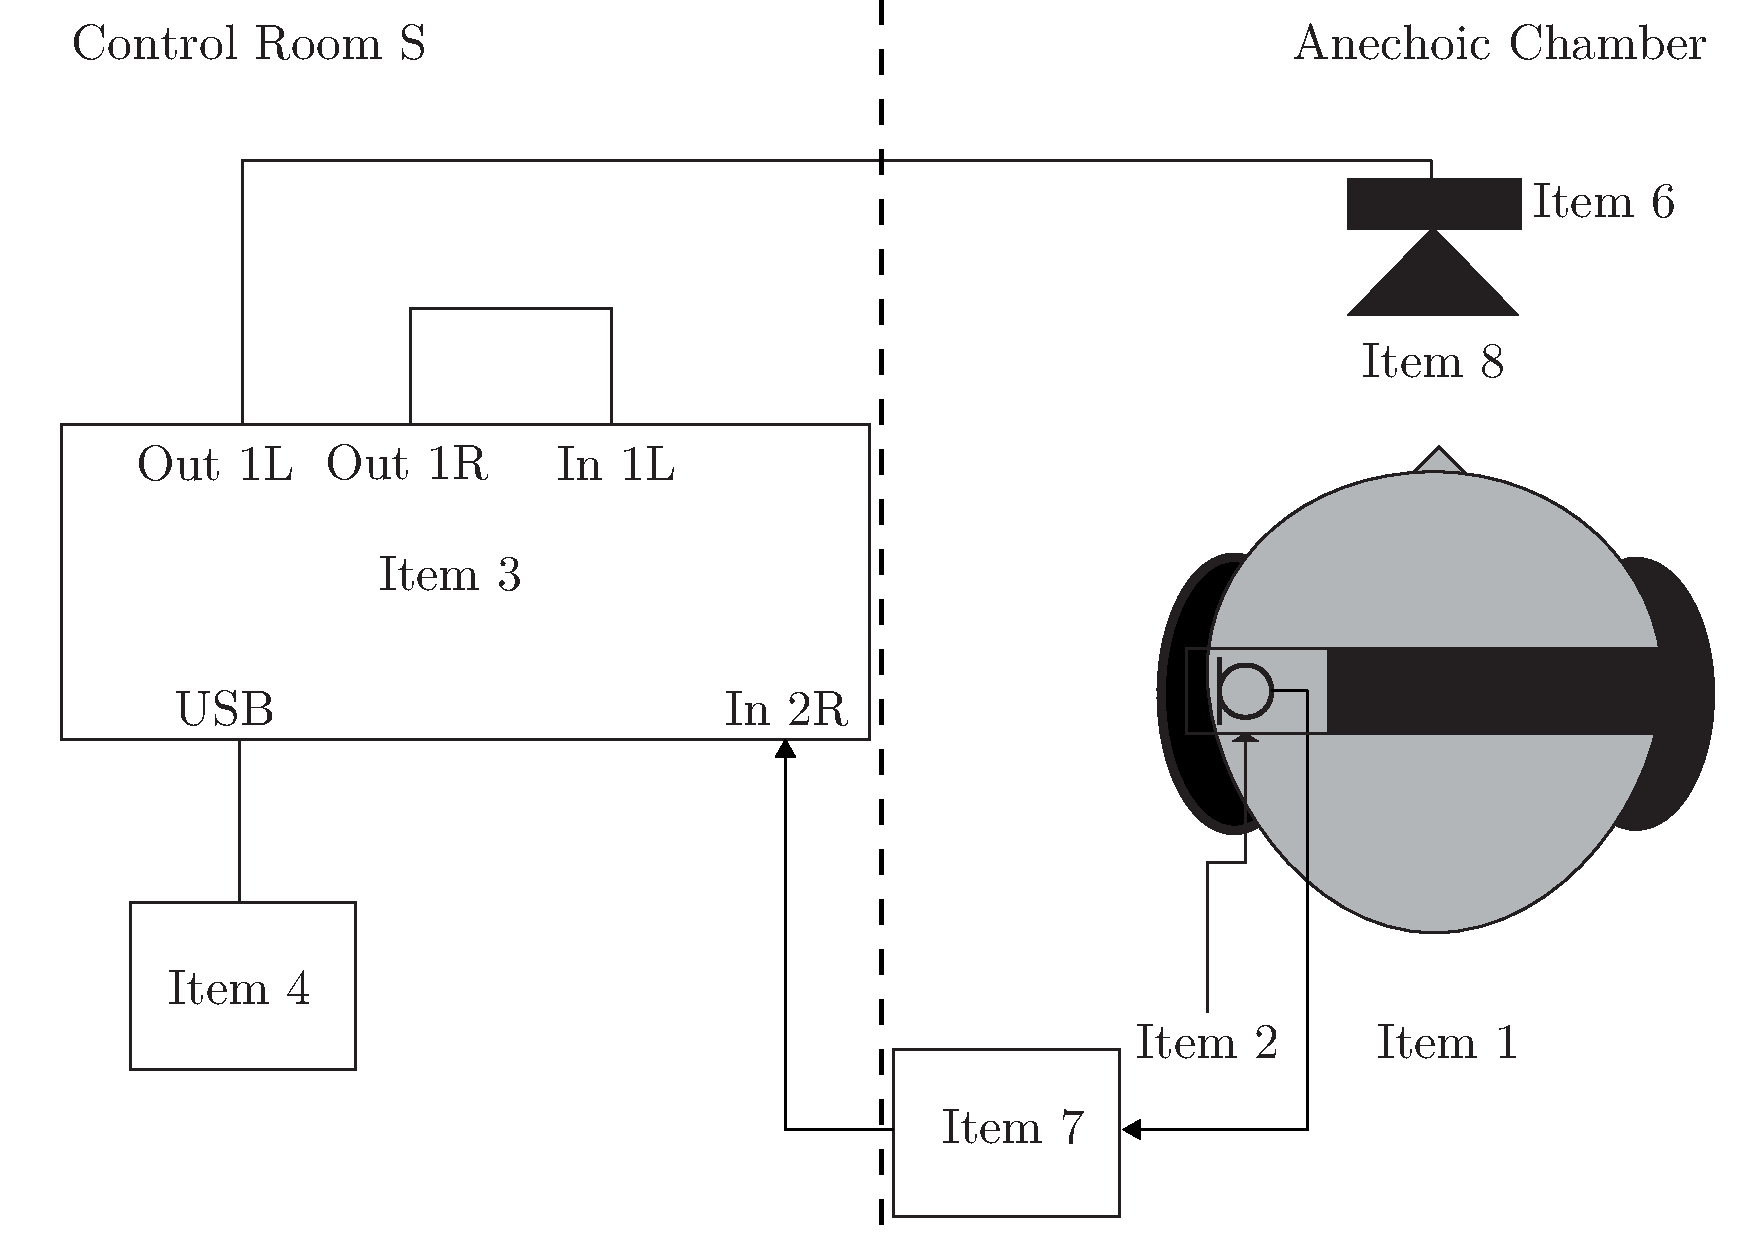
\includegraphics[width=0.8\textwidth]{../Journal/Experiments/TestofConsumerHeadphones/OtherBrandsDiagram.pdf}
	\caption{Diagram of the test set-up.}
	\label{OtherBrandsDiagram}
\end{figure}

\subsection{Settings/Description}
\subsubsection{Control and calibration}
\begin{itemize}
	\item Item 6  is placed 1.6 meters from the Item 1.
	\item Item 2 calibrations are made on the computer using Simulink\textsuperscript{\textregistered}.
	\begin{itemize} 
		\item Calibration is made @ 1 $k$Hz using Item 5 with adapter for Item 2. This should yield a signal of 95.6 dB. The measured intensity in MATLAB\textsuperscript{\textregistered} however was 78.12 so all measurements are multiplied by 7.48 to get a calibrated signal in Matlab\textsuperscript{\textregistered}.
	\end{itemize}
\end{itemize}

\subsubsection{Equipment settings}
\begin{itemize}
	\item This experiment is performed with a sampling rate, $F_{s}$ = 48 $k$Hz. 
	\item For Item 5 take care to turn on the "inst"-option in the mixing console. The following gain settings are present: 		
	\begin{itemize}
		\item Line level gain is 0 dB
		\item Error Microphones has gain +30 dB
		\item Ref Microphones has gain +48 dB
		\item Speaker Microphones has gain +48 dB
	\end{itemize}
	\item All settings on the computer is set to 0 dBFS
\end{itemize}
	
	
\subsection{Picture}
\begin{figure}[H]
	\centering
	\begin{subfigure}[b]{0.5\textwidth}
		\centering
		%	\tikzsetnextfilename{AttenuationSetup}
		%	
\definecolor{cffffff}{RGB}{255,255,255}

\resizebox {0.4\columnwidth} {!} {
\begin{tikzpicture}[y=0.80pt, x=0.80pt, yscale=-1.000000, xscale=1.000000, inner sep=0pt, outer sep=0pt]
\begin{scope}% layer1
  % text3396
  \path[fill=black,line join=miter,line cap=butt,line width=0.800pt]
    (242.8571,610.2194) node[above right] (text3396) {};

  % rect5654
  \path[draw=black,fill=cffffff,opacity=0.980,miter limit=4.00,line
    width=0.837pt,rounded corners=0.0000cm] (0.0000,492.3622) rectangle
    (460.0000,1052.3622);

  % path5656
  \path[draw=black,dash pattern=on 2.40pt off 0.80pt,line join=miter,line
    cap=butt,miter limit=4.00,even odd rule,line width=0.800pt] (0.0000,482.3622)
    .. controls (460.0000,482.3622) and (460.0000,482.3622) ..
    (460.0000,482.3622);

  % path6121
  \path[draw=black,dash pattern=on 2.40pt off 0.80pt,line join=miter,line
    cap=butt,miter limit=4.00,even odd rule,line width=0.800pt]
    (470.0000,1052.3622) -- (470.0000,492.3622);

  % rect6329
  \path[draw=black,fill=cffffff,opacity=0.980,miter limit=4.00,line
    width=0.800pt,rounded corners=0.0000cm] (220.1005,972.3622) rectangle
    (260.1005,1012.3622);

  % rect6329-8
  \path[draw=black,fill=cffffff,opacity=0.980,miter limit=4.00,line
    width=0.800pt,rounded corners=0.0000cm] (50.3174,692.3748) rectangle
    (90.3174,732.3748);

  % rect6329-8-5
  \path[draw=black,fill=cffffff,opacity=0.980,miter limit=4.00,line
    width=0.800pt,rounded corners=0.0000cm] (370.6172,692.3992) rectangle
    (410.6172,732.3992);

  % rect6329-8-1
  \path[draw=black,fill=cffffff,opacity=0.980,miter limit=4.00,line
    width=0.800pt,rounded corners=0.0000cm] (220.0700,651.8595) rectangle
    (260.0700,691.8595);

  % path6381
  \path[draw=black,fill=cffffff,opacity=0.980,miter limit=4.00,line width=0.800pt]
    (239.6594,819.1820) circle (0.4233cm);

  % path6695
  \path[draw=black,dash pattern=on 2.40pt off 0.80pt,line join=miter,line
    cap=butt,miter limit=4.00,even odd rule,line width=0.800pt] (50.0000,732.3622)
    -- (50.0000,1052.3622);

  % path6697
  \path[draw=black,dash pattern=on 2.40pt off 0.80pt,line join=miter,line
    cap=butt,miter limit=4.00,even odd rule,line width=0.800pt] (0.0000,692.3622)
    -- (220.0000,692.3622) -- (220.0000,1052.3622);

  % path6699
  \path[draw=black,dash pattern=on 2.40pt off 0.80pt,line join=miter,line
    cap=butt,miter limit=4.00,even odd rule,line width=0.800pt]
    (370.0000,732.3622) -- (0.0000,732.3622);

  % text4186
  \path[cm={{0.0,-1.0,1.0,0.0,(0.0,0.0)}},fill=black,line join=miter,line
    cap=butt,line width=0.800pt] (-1049.0592,215.0796) node[above right,rotate=90]
    (text4186) {16 cm};

  % text4186-3
  \path[cm={{0.0,-1.0,1.0,0.0,(0.0,0.0)}},fill=black,line join=miter,line
    cap=butt,line width=0.800pt] (-926.5287,234.3933) node[above right,rotate=90]
    (text4186-3) {15 cm};

  % text4186-1
  \path[fill=black,line join=miter,line cap=butt,line width=0.800pt]
    (252.8320,728.8373) node[above right] (text4186-1) {14 cm};

  % text4186-2
  \path[fill=black,line join=miter,line cap=butt,line width=0.800pt]
    (89.1852,688.5429) node[above right] (text4186-2) {13 cm};

  % text4186-4
  \path[fill=black,line join=miter,line cap=butt,line width=0.800pt]
    (1.3101,746.2242) node[above right] (text4186-4) {12 cm};

  % text4186-0
  \path[cm={{0.0,-1.0,1.0,0.0,(0.0,0.0)}},fill=black,line join=miter,line
    cap=butt,line width=0.800pt] (-914.2587,63.6862) node[above right,rotate=90]
    (text4186-0) {11 cm};

  % text4186-3-8
  \path[cm={{0.0,-1.0,1.0,0.0,(0.0,0.0)}},fill=black,line join=miter,line
    cap=butt,line width=0.800pt] (-781.0693,486.7263) node[above right,rotate=90]
    (text4186-3-8) {10 cm};

  % text4186-3-6
  \path[fill=black,line join=miter,line cap=butt,line width=0.800pt]
    (203.8091,475.7764) node[above right] (text4186-3-6) {17 cm};

  % text4186-2-1
  \path[fill=black,line join=miter,line cap=butt,line width=0.800pt]
    (63.7294,718.4424) node[above right] (text4186-2-1) {A};

  % text4186-2-1-2
  \path[fill=black,line join=miter,line cap=butt,line width=0.800pt]
    (232.8284,677.5307) node[above right] (text4186-2-1-2) {B};

  % text4186-2-1-9
  \path[fill=black,line join=miter,line cap=butt,line width=0.800pt]
    (385.7573,717.3333) node[above right] (text4186-2-1-9) {C};

  % text4186-2-1-6
  \path[fill=black,line join=miter,line cap=butt,line width=0.800pt]
    (233.8228,997.7496) node[above right] (text4186-2-1-6) {D};

  % text4326
  \path[fill=black,line join=miter,line cap=butt,line width=0.800pt]
    (233.0000,826.8622) node[above right] (text4326) {1};

\end{scope}

\end{tikzpicture}}


		\includegraphics[width=\textwidth]{../Journal/Experiments/TestofConsumerHeadphones/Pictures/OtherBrandsSetupBack.jpg}
		\caption{Set-up from the back.}
		%\label{fig:AttenuationSetup}
	\end{subfigure}\qquad
	\begin{subfigure}[b]{0.4\textwidth}
		\includegraphics[width=\textwidth]{../Journal/Experiments/TestofConsumerHeadphones/Pictures/OtherBrandsSetupAngle.jpg}
		\caption{Set-up form an angle.}
		%\label{fig:SetupFront}
		\vspace{2ex}
		\includegraphics[width=\textwidth]{../Journal/Experiments/TestofConsumerHeadphones/Pictures/OtherBrandsSetupSide.jpg}
		\caption{Set-up form the side.}
		%\label{fig:SetupBack}
	\end{subfigure}
	\caption{The test set-up form different angles with the Bose QuietComfort 25 headphone.}
\label{fig:OtherBrandsPicture}
\end{figure}


\subsection{Procedure}
	\subsubsection{Set-up}
	\begin{enumerate}
		\item Connect cable from Item 3's "Out 1L" to Item 6's "Line in"
		\item Connect cable from Item 3's "Out 1R" to Item 3's "In 1L"
		\item Connect cable from Item 2 to Item 7's "Input"
		\item Connect cable from Item 7's "Output" to Item 3's "IN 2R"
		\item Connect USB-cable from Item 4 to Item 3
	\end{enumerate}

	\subsubsection{Performing Experiment}
	\begin{enumerate}
		\item Open Simulink\textsuperscript{\textregistered} and open and run file \path{OtherBrands.xls}
		\begin{itemize} 
			\item The simulations outputs a speech signal at 0 dBFS over the span of 12 seconds
			\begin{itemize}
				\item [] The signal constructed using speech-files from "The Archimedes Project" by Bang \& Olufsen. \\
				The signal is composed of three seconds of the UK male anechoic sample followed by three seconds of silence, followed by the UK female anechoic sample, and ends with another three seconds of silence.
			\end{itemize}
			\item The simulation runs for 14 seconds
		\end{itemize}
		\item Rename generated file \path{GeneratedANC} according to headphone tested, and whether or not ANC was enabled. E.g. \path{Denonon[1].wav} for the first test of the Denon AH GC20 headhpone with ANC enabled. Names in \path{evaluatePerformance.m}-script is named accordingly.
				\begin{itemize}
			\item[] Perform this experiment for as many headphones as desired.
		\end{itemize}
	\end{enumerate}
	
		
\subsection{Data Extraction}
\begin{enumerate}
	\item Open MATLAB\textsuperscript{\textregistered} and run script \path{evaluatePerformance.m}
\end{enumerate}

From performing the experiment, a list of files were generated, ten for each device tested; five with ANC enabled and five with ANC disabled.
The difference between the enabled and the disabled is plotted on the graph below, for each device tested. The list can be seen below

\begin{itemize}
	\item \path{Denonon[i].wav}			(Denon AH GC20 w/ ANC)
	\item \path{Denonoff[i].wav}		(Denon AH GC20 w/o ANC)
	\item \path{BoseQC15on[i].wav}		(Bose QuietComfort 15 w/ ANC)
	\item \path{BoseQC15off[i].wav}		(Bose QuietComfort 15 w/o ANC)
	\item \path{BoseQC25on[i].wav}		(Bose QuietComfort 25 w/ ANC)
	\item \path{BoseQC25off[i].wav}		(Bose QuietComfort 25 w/o ANC)
	\item \path{BOH8on[i].wav}			(B\&O BEOPLAY H8 w/ ANC)
	\item \path{BOH8off[i].wav}			(B\&O BEOPLAY H8 w/o ANC)
	\item \path{Denonon[i].wav}		(Denon AH GC20 w/ ANC)
	\item "Denonoff[i].wav"		(Denon AH GC20 w/o ANC)
	\item "BoseQC15on[i].wav"		(Bose QuietComfort 15 w/ ANC)
	\item "BoseQC15off[i].wav"		(Bose QuietComfort 15 w/o ANC)
	\item "BoseQC25on[i].wav"		(Bose QuietComfort 25 w/ ANC)
	\item "BoseQC25off[i].wav"		(Bose QuietComfort 25 w/o ANC)
	\item "BOH8on[i].wav"			(B\&O BEOPLAY H8 w/ ANC)
	\item "BOH8off[i].wav"		(B\&O BEOPLAY H8 w/o ANC)
	\footnote{[i] indicates the iteration of the experiment}
\end{itemize}


\subsection{Analysis}
The five files of each ANC setting for each headphone is then meaned and cross correlated with the opposing ANC-setting of the same headphone, to find the relative difference between the headphones on- and off ANC-setting.\\
This difference is then plotted for all headphones on \autoref{fig:OtherBrandsTestCompare}.
\\
The impulse response of the difference between enabled and disabled recorded signals is to be found.
This is done by finding the frequency response of the "signal", which the cross correlation between e.g. \path{Denonon[i].wav} and \path{Denonon[i].wav} This is done by taking the FT of the cross correlated signals, seen in \autoref{FrequencyResponseEq2}.


\begin{equation}\label{FrequencyResponseEq2}
%H(f) = \frac{Y(m_{\mu}) *  X(r_{\mu})}{X(r_{\mu}) *  X(r_{\mu})}
H(f) = \frac{Y(f) \cdot X\textsuperscript{*}(f)}{X(f) \cdot X\textsuperscript{*}(f)}
\end{equation}
Where:
\begin{itemize}
	%\item " $*$ " denotes the complex conjugation
	\item $H(f)$ is the FT of the 'Difference between the signals'
	\item $Y(f)$ is the FT of the recorded signals, with ANC enabled,  Denonon[i]
	\item $X(f)$ is the FT of the recorded signals, with ANC disabled, Denonoff[i]
\end{itemize}

\begin{figure}[H]
	\centering
	\begin{subfigure}[b]{.48\textwidth}
	\centering
	\includegraphics[width=1\textwidth]{../Article/tikz/ComparedConusmerHPAppSub1}
	\end{subfigure}
%	\hfill
	\begin{subfigure}[b]{.48\textwidth}
		\centering
	\includegraphics[width=1\textwidth]{../Article/tikz/ComparedConusmerHPAppSub2}
	\end{subfigure}
	\begin{subfigure}[b]{.48\textwidth}
	\centering
	\includegraphics[width=1\textwidth]{../Article/tikz/ComparedConusmerHPAppSub3}
	\end{subfigure}
%	\hfill
	\begin{subfigure}[b]{.48\textwidth}
	\centering
	\includegraphics[width=1\textwidth]{../Article/tikz/ComparedConusmerHPAppSub4}
	\end{subfigure}
\end{figure}


<<<<<<< HEAD
\begin{figure}[H]
	\centering
	\tikzsetnextfilename{ComparedConusmerHPApp}
	\input{../Journal/Experiments/TestofConsumerHeadphones/Plots/SmoothCompareAppendix(fig).tex}
	\caption{Denon, B\&O H8 Bose QC15 Bose QC25.}
	\label{fig:OtherBrandsTestCompare}
\end{figure}
=======
%\begin{figure}[H]
%	\centering
%	\tikzsetnextfilename{ComparedConusmerHP}
%	\input{../Journal/Experiments/TestofConsumerHeadphones/Plots/SmoothCompareAppendix(fig).tex}
%	\caption{Denon (blue), B\&O H8 (red) Bose QC15 (Yellow) Bose QC25 (Purple).}
%	\label{fig:ANCcompare}
%\end{figure}
>>>>>>> 73d5ce9ed1ed059396c4ad9c248ae93afc444a71

\subsection{Conclusion}
The relative difference between a headphones attenuation with and without ANC was found for four different consumer headphones.


\begin{figure}[H]
	\centering
	\tikzsetnextfilename{ComparedConusmerHPAppSub4}
	\input{../Journal/Experiments/TestofConsumerHeadphones/Plots/CunsumerHpSubplot4(fig).tex}
	\caption{Denon, B\&O H8 Bose QC15 Bose QC25.}
	\label{fig:OtherBrandsTestCompare}
\end{figure}



